\section{Python Application}

\subsection{Architecture}
The Hospital Management System utilizes a modular, three-tier client-server architecture to ensure efficient data flow and separation of concerns:
\begin{itemize}
    \item \textbf{Presentation Layer:} A frontend built with HTML, CSS, and vanilla JavaScript (\texttt{index.html, style.css, app.js}) that uses the asynchronous \texttt{fetch()} API to execute CRUD operations seamlessly without page reloads.
    \item \textbf{Application Layer:} A Python Flask backend (\texttt{main.py}) exposing a RESTful API \cite{flask_docs, flask_quickstart}. It encapsulates business logic (\texttt{operations.py}), handles report generation (\texttt{reports.py}), and normalizes complex database types into JSON format for the client.
    \item \textbf{Data Layer:} A MySQL database connected via \texttt{mysql-connector-python} (\texttt{database.py}). It houses five core tables (Patients, Doctors, Departments, Appointments, and Invoices) and leverages Stored Procedures, Triggers, and Views to automate workflows, ensure data integrity, and streamline reporting.
\end{itemize}

\begin{figure}[H]
    \centering
    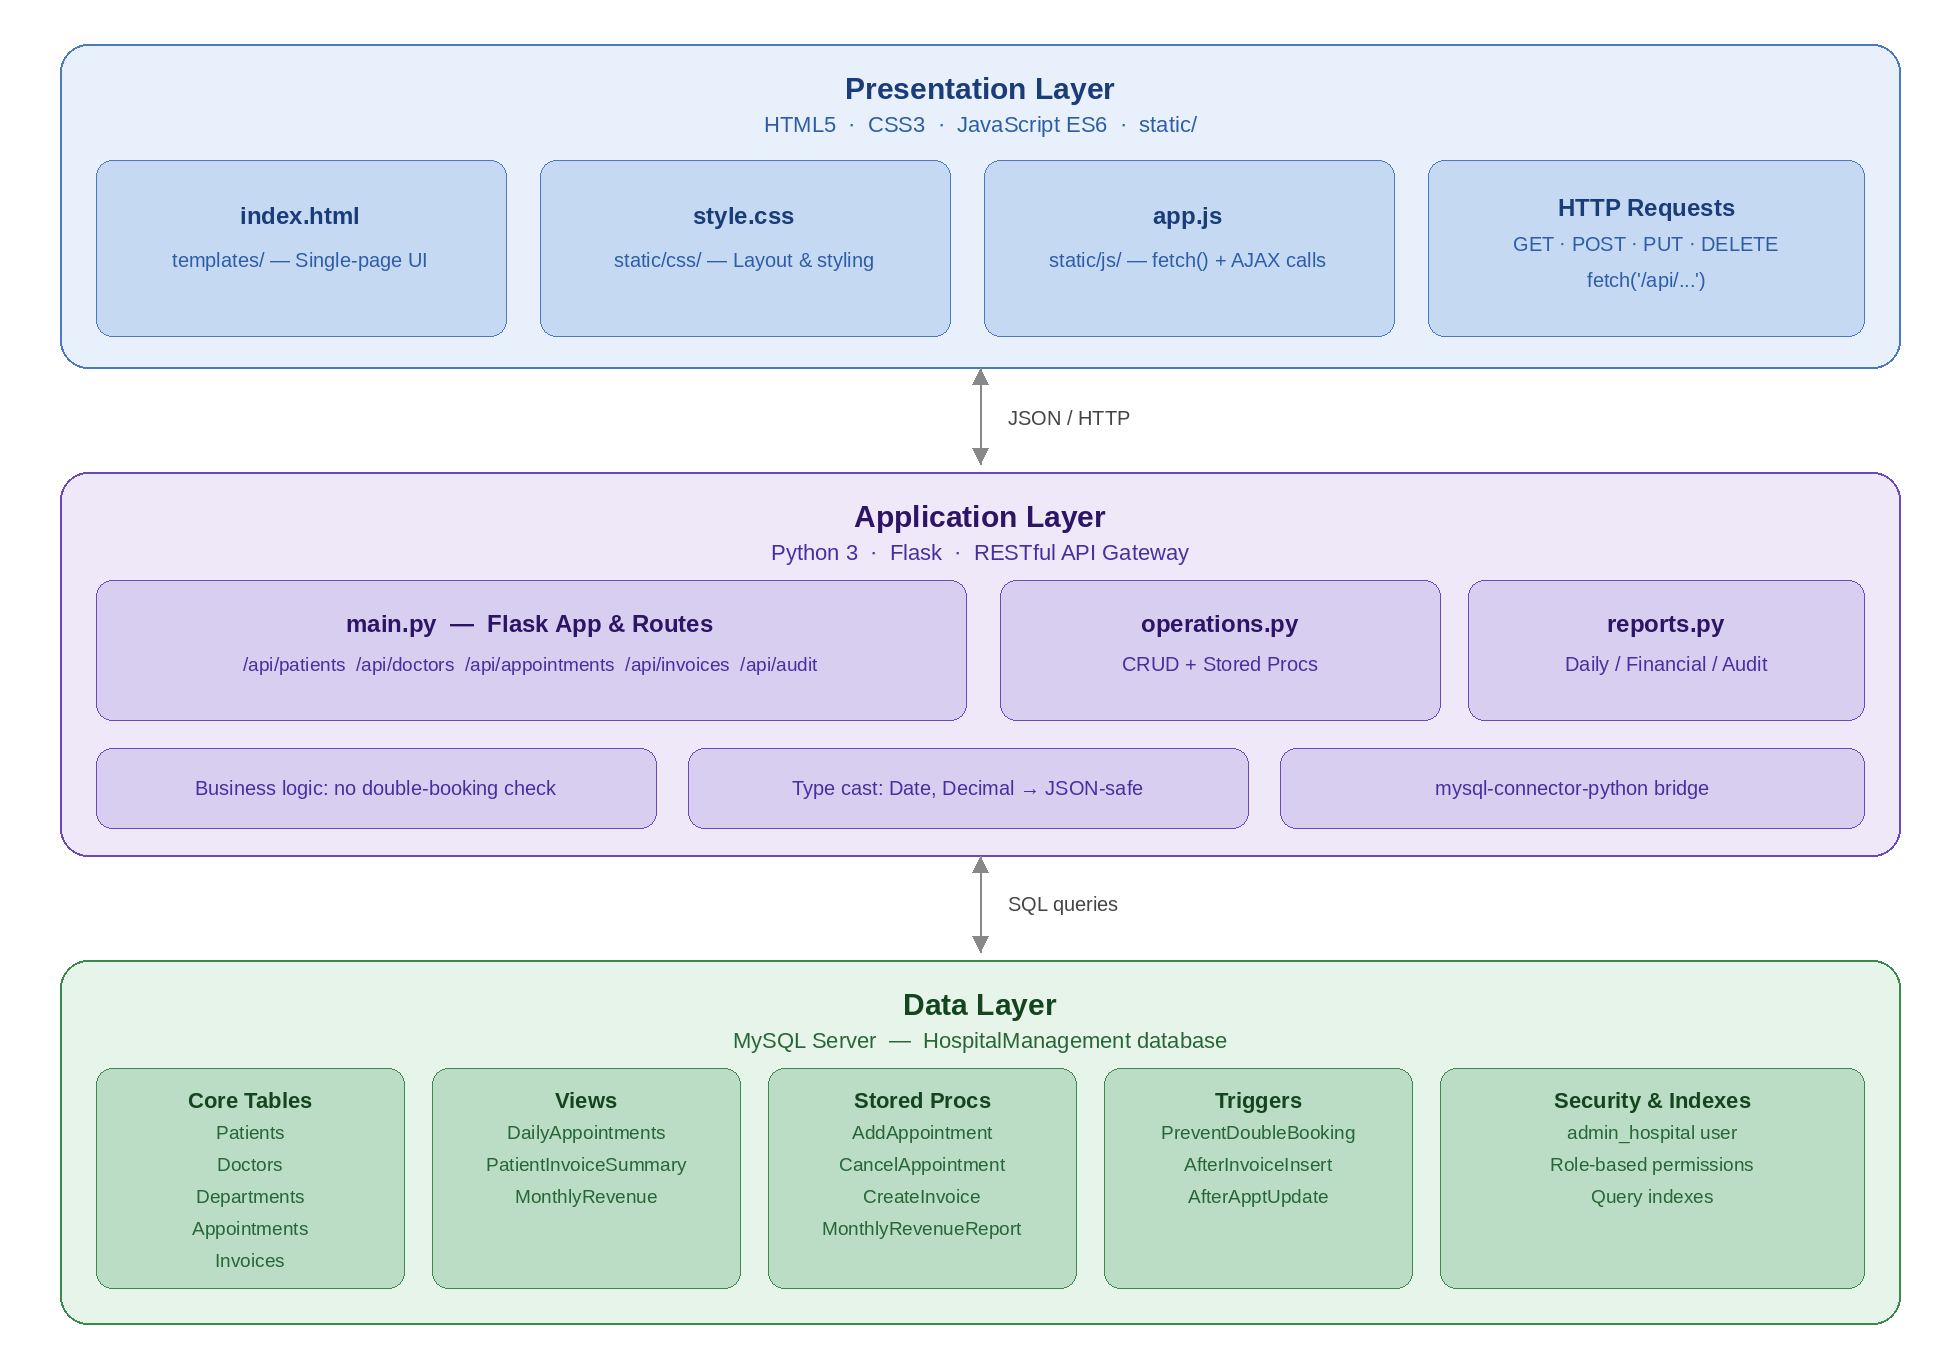
\includegraphics[width=1\textwidth]{Images/hms_architecture_v2.png}
    \caption{Systen Architecture}
    \label{fig:sys_architecture}
\end{figure}

The complete source code for this project, including all Python application files, SQL scripts, and frontend assets, is publicly available at: \texttt{https://github.com/manhh05/hospital-management-system}

\subsection{Database Integration}
The application utilizes the \texttt{mysql-connector-python} library to bridge the Python backend with the MySQL server \cite{mysql_connector_guide}. This integration focuses on security, modularity, and efficient data handling.

\subsubsection*{Connectivity and Session Management}
All database interactions are initiated via a centralized \texttt{connect\_to\_database()} function. This entry point establishes a connection using dedicated credentials, ensuring isolated operations for every request
\begin{pythoncode}
def connect_to_database():
    connection = mysql.connector.connect(
        host='localhost',
        database='HospitalManagement',
        user='admin_hospital',
        password='AdminPass123'
    )
    return connection
\end{pythoncode}

\begin{itemize}
    \item To prevent resource leaks, each operation follows a strict pattern of opening a connection at the start and releasing it within a \texttt{finally} block, ensuring high system availability
\end{itemize}

\subsubsection*{CRUD and Data Handling}
\begin{itemize}
    \item \textbf{Parameterized Queries:} Standard data management (Create, Read, Update, Delete) is performed using parameterized queries with \texttt{\%s} placeholders to prevent SQL injection
    \item \textbf{Dictionary Cursors:} The system employs \texttt{cursor(dictionary=True)} for read operations, allowing the Flask application to access fields by column name rather than raw tuples \cite{mysql_connector_connecting}.
    \item \textbf{Type Normalization:} Before returning JSON responses, the application normalizes MySQL-specific types, such as converting \texttt{Date} to strings and \texttt{Decimal} values to floats, to ensure compatibility with Flask's \texttt{jsonify}
\end{itemize}

\subsubsection*{Stored Procedure Execution}
For complex transactional workflows, the application delegates logic to MySQL stored procedures using the \texttt{cursor.callproc()} method. This approach keeps business logic close to the data and ensures atomic operations
\begin{pythoncode}
def schedule_appointment(doctor_id, patient_id, appt_date, appt_time):
    conn = connect_to_database()
    cursor = conn.cursor()
    
    cursor.callproc('AddAppointment', (doctor_id, patient_id, appt_date, appt_time))
    conn.commit()
\end{pythoncode}

This architecture allows the application to retrieve \texttt{OUT} parameters, such as newly generated IDs, directly from the database without requiring additional queries.

\subsection{Core Features}

The application provides five functional modules, each integrated with a dedicated API endpoint and specific database logic to ensure operational consistency

\begin{itemize}
    \item \textbf{Patient Management:} Facilitates full CRUD operations (Create, Read, Update, Delete) through the \texttt{/api/patients} endpoint. It includes a search utility to retrieve patient details by ID, which is essential for streamlining appointment and invoice creation.
    \item \textbf{Doctor Management:} Manages comprehensive doctor profiles—including specialties and department assignments, via the \texttt{/api/doctors} endpoint. Relational integrity is maintained through foreign keys linked to the \texttt{Departments} table.
    \item \textbf{Appointment Scheduling:} Utilizes the \texttt{AddAppointment} stored procedure to manage scheduling. The system enforces the \texttt{PreventDoubleBooking} trigger to reject conflicting slots at the database level. Cancellations are processed via \texttt{CancelAppointment}, which automatically updates the audit trail through the \texttt{AfterAppointmentUpdate} trigger.
    \item \textbf{Invoice Management:} Implements the \texttt{CreateInvoice} stored procedure to handle financial transactions. This procedure executes a single transaction that inserts the invoice, updates the patient's last payment date, and records an audit entry. The \texttt{/api/invoices} endpoint normalizes all financial data to ensure compatibility with the frontend.
    \item \textbf{Audit Logging:} Provides transparency through the \texttt{/api/audit} endpoint, which exposes the \texttt{AuditLog} table. Logging is largely automated via database triggers to ensure that key events,such as invoice creation and appointment status changes—are recorded consistently, regardless of how the data is accessed.
\end{itemize}

\subsection{Reporting Module}

The reporting module, implemented in \texttt{reports.py}, provides high-level data insights by querying pre-built database views and executing complex stored procedures. Each function follows a consistent connection pattern, returning results as dictionaries to facilitate seamless JSON serialization for the web interface.
\begin{itemize}
    \item \textbf{Daily Appointments Report:} The \texttt{get\_daily\_appointments\_report()} function queries the \texttt{DailyAppointments} view, which joins the Patients, Doctors, and Departments tables. This report displays comprehensive schedule details, with status values: Scheduled, Completed, or Cancelled—automatically, managed by the \texttt{AfterAppointmentUpdate} trigger.
    \begin{figure}[H]
        \centering
        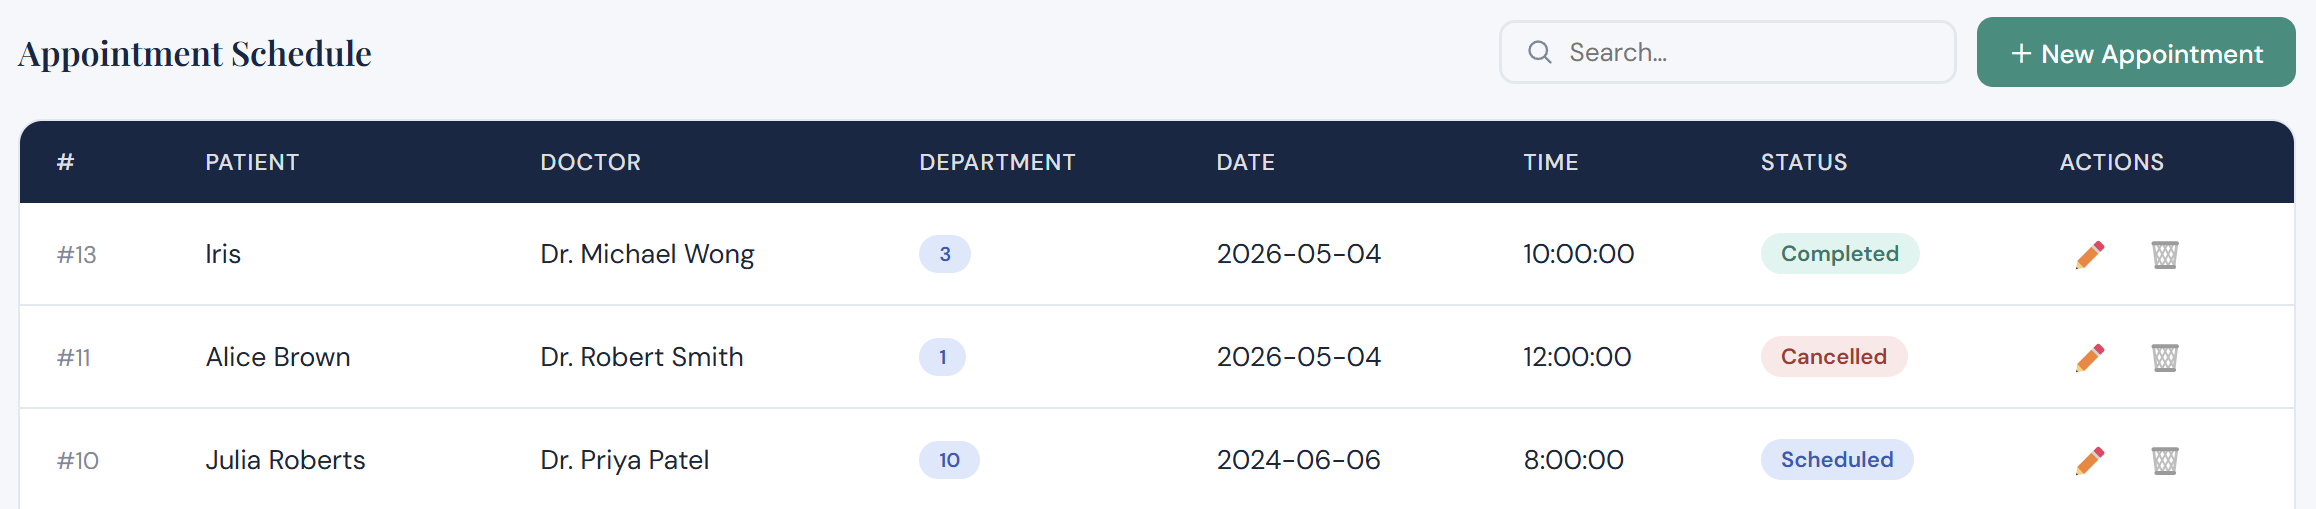
\includegraphics[width=0.8\textwidth]{Images/web_appointment_schedule.png}
        \caption{Appointment Schedule as rendered in the web interface}
        \label{fig:web_appointment_schedule}
    \end{figure}
    \item \textbf{Financial Summary and Invoice Report:} Utilizing the \texttt{PatientInvoiceSummary} view via \texttt{get\_financial\_summary()}, the system aggregates billing data on a per-patient basis. While the backend provides raw invoice data and payment statuses (Paid, Partially Paid, Unpaid), the frontend applies a 10\% surcharge calculation for tax-inclusive figures.
    \begin{figure}[H]
        \centering
        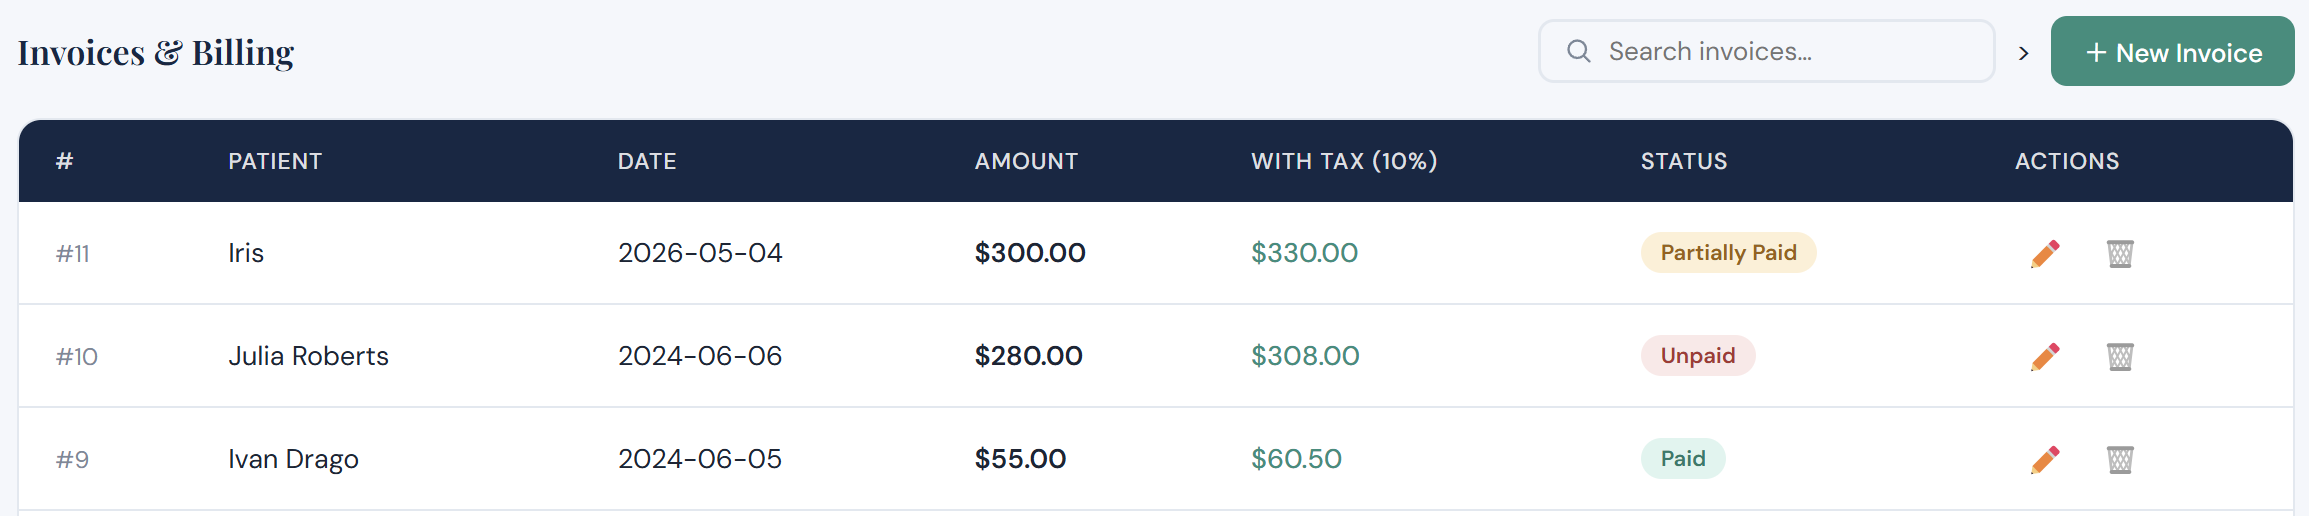
\includegraphics[width=0.8\textwidth]{Images/web_invoice_billing.png}
        \caption{Invoices \& Billing as rendered in the web interface}
        \label{fig:web_invoice_billing}
    \end{figure}
    \item \textbf{Monthly Revenue Report:} The \texttt{get\_monthly\_revenue\_report(year, month)} function executes the \texttt{MonthlyRevenueReport} stored procedure. It generates two distinct result sets: a granular breakdown of individual invoices and a high-level summary of gross revenue, collected funds, and outstanding balances.
    \item \textbf{Patient Visit Statistics:} Administered through \texttt{get\_patient\_statistics()}, this module performs a multi-table JOIN across Departments, Doctors, and Appointments. It calculates visit frequencies per department, sorted by volume, to provide administrators with a clear overview of departmental workload distribution.
\end{itemize}

\subsection{User Interface (CLI/GUI)}

\begin{figure}[H]
    \centering
    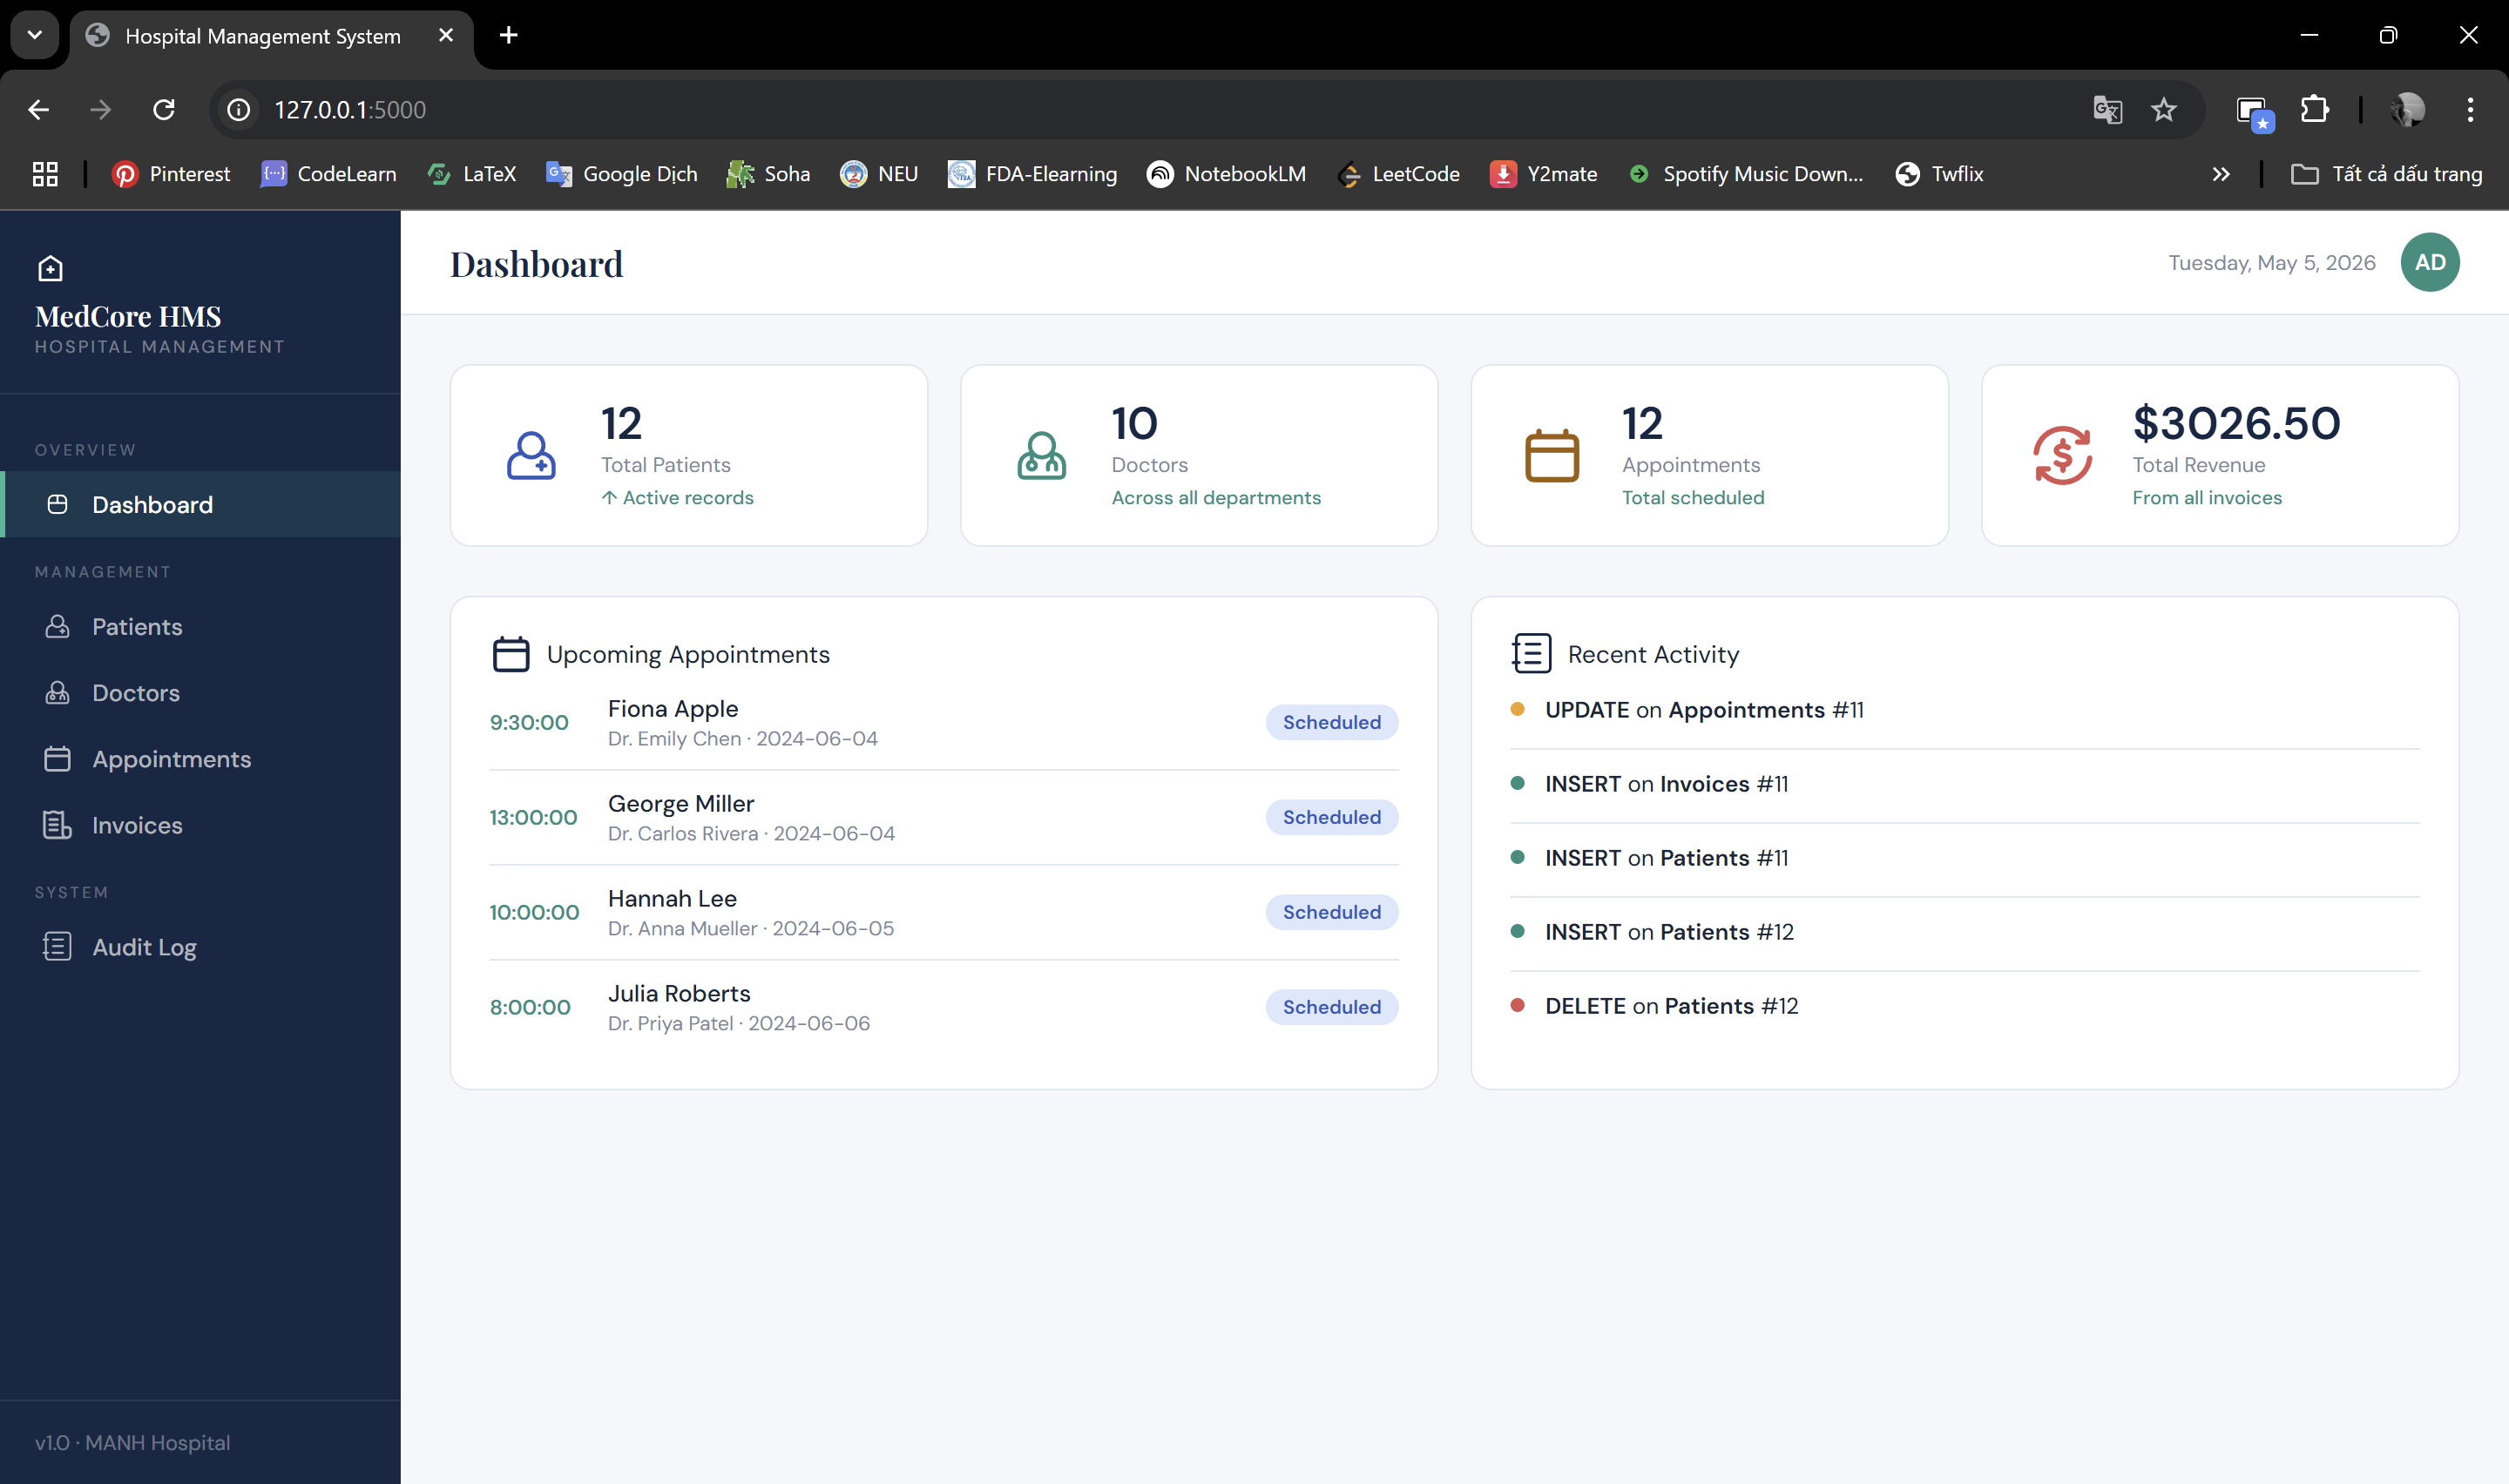
\includegraphics[width=1\textwidth]{Images/web_dashboard.png}
    \caption{Dashboard in the web interface}
    \label{fig:web_dashboard}
\end{figure}

\begin{figure}[H]
    \centering
    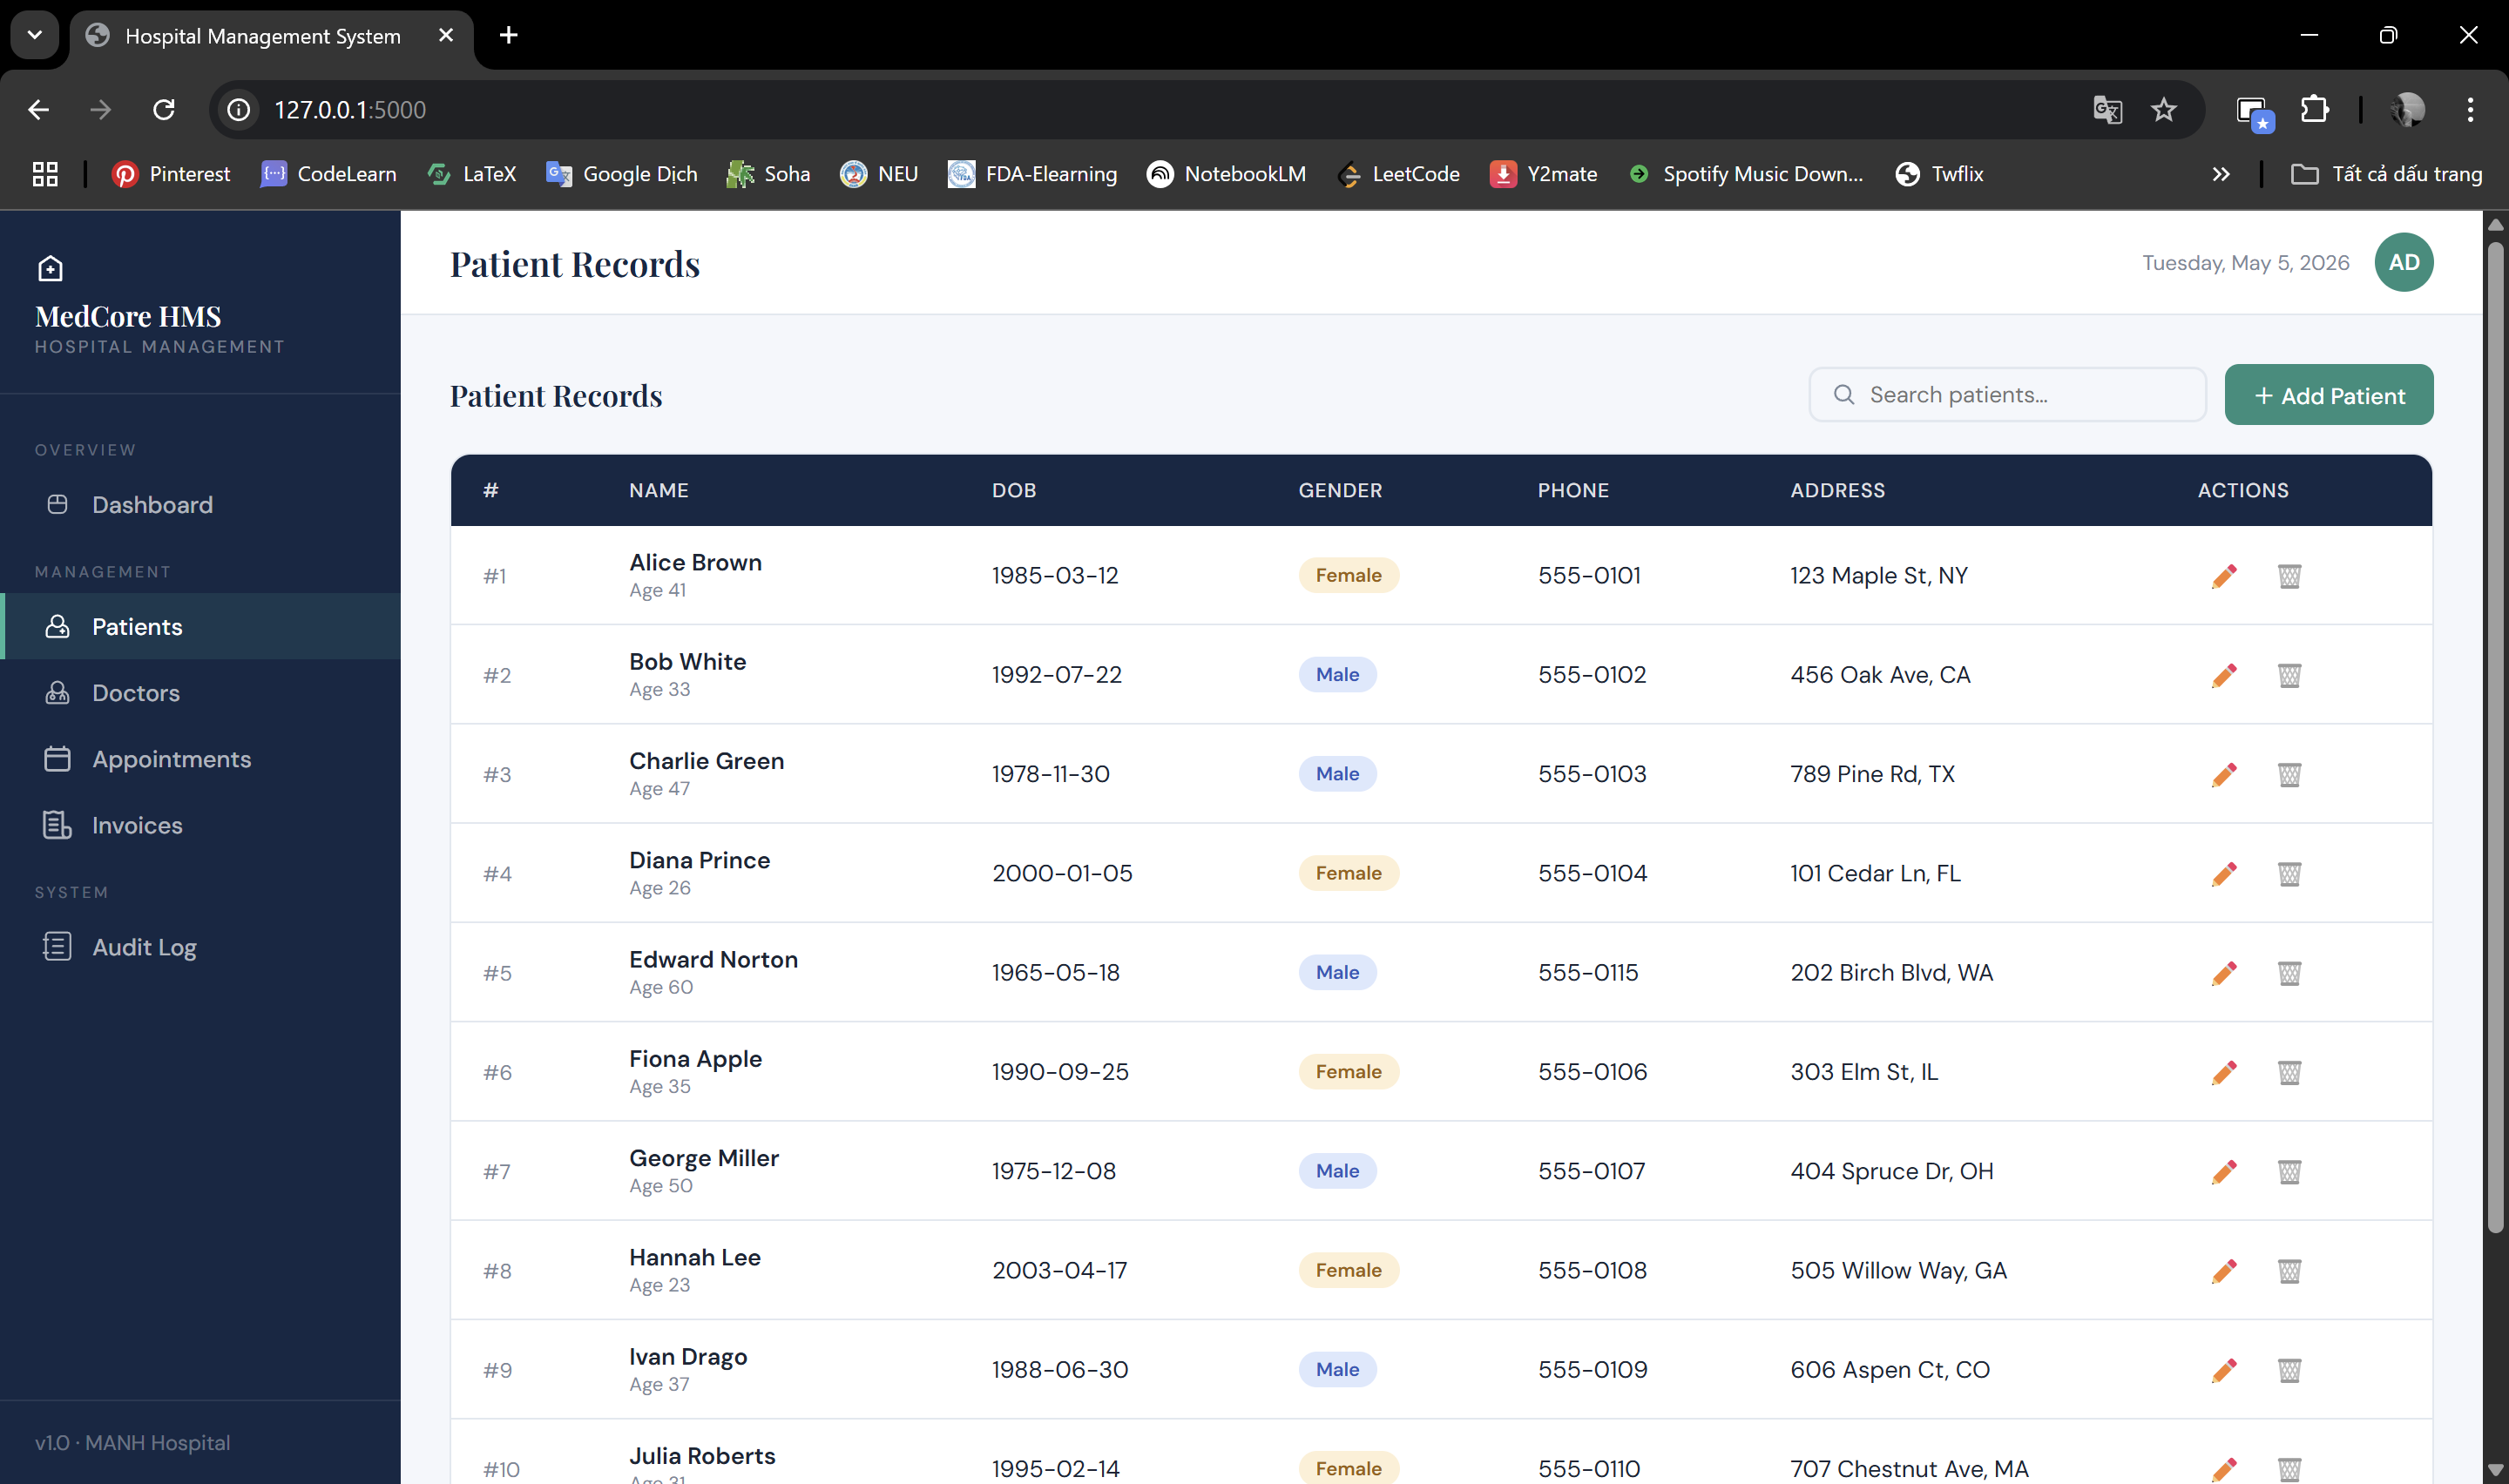
\includegraphics[width=1\textwidth]{Images/web_patients.png}
    \caption{Patients Management in the web interface}
    \label{fig:web_patients}
\end{figure}

\begin{figure}[H]
    \centering
    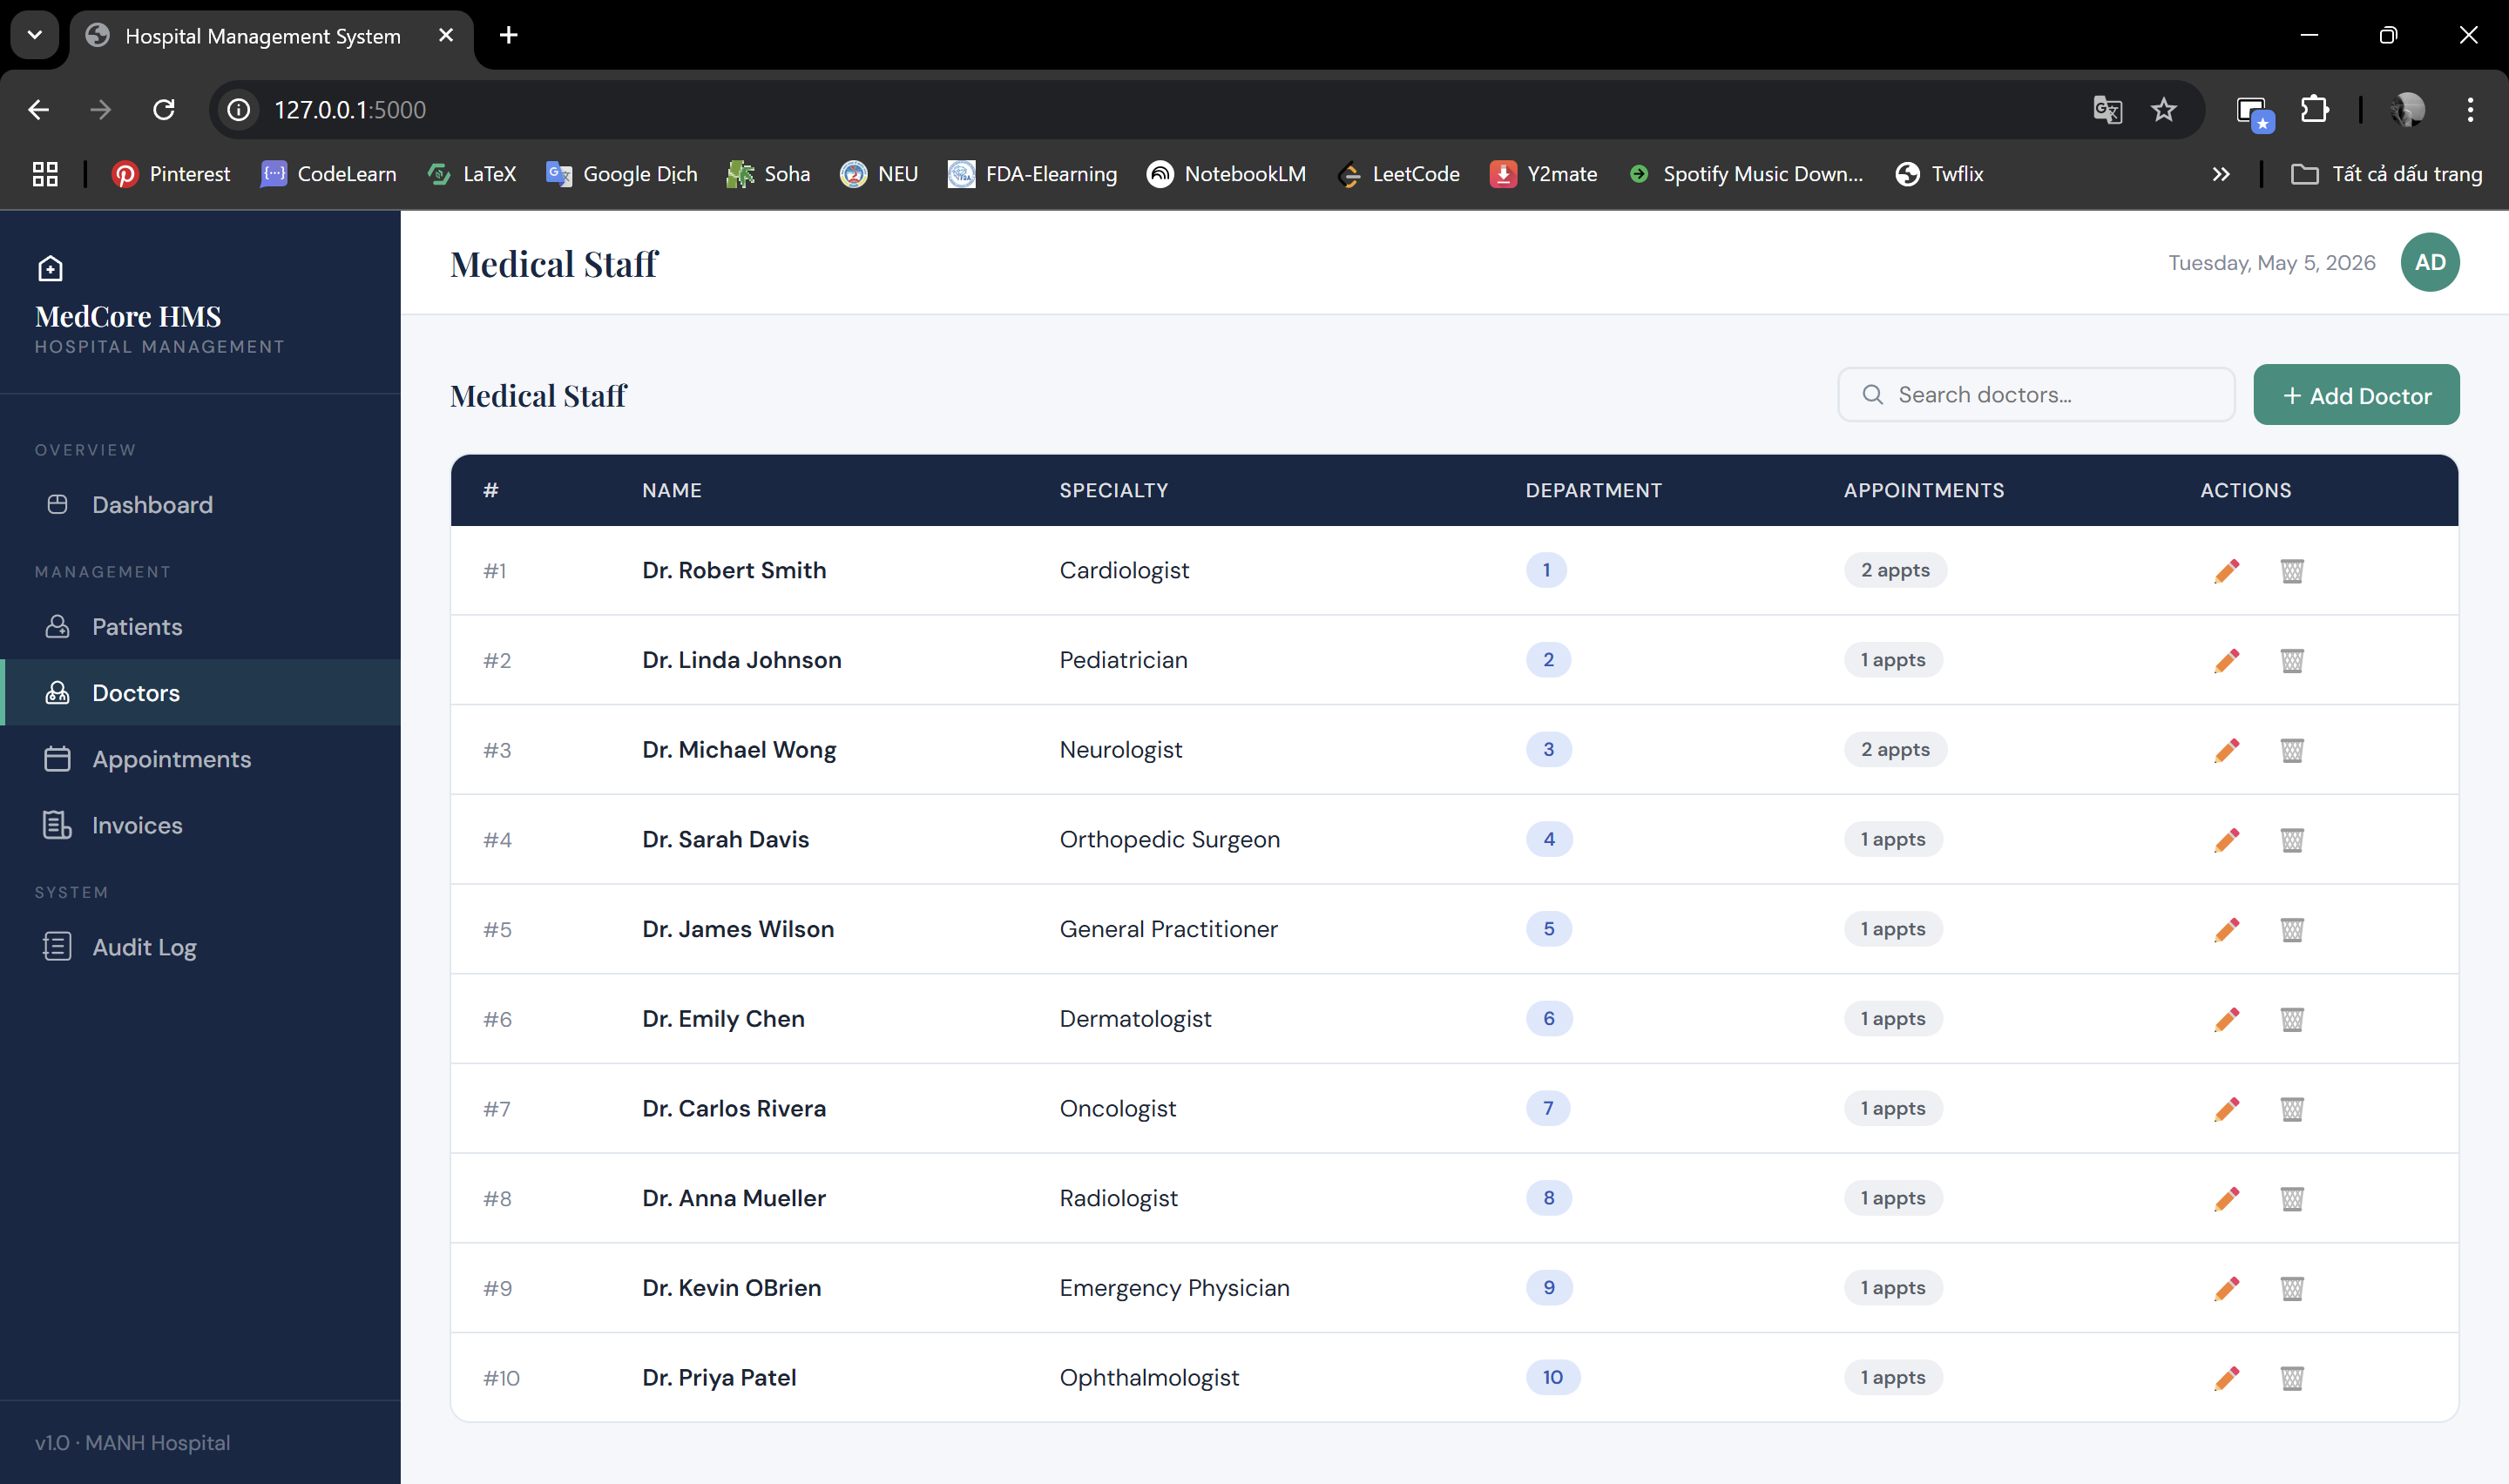
\includegraphics[width=1\textwidth]{Images/web_doctors.png}
    \caption{Doctors in the web interface}
    \label{fig:web_doctors}
\end{figure}